% !TEX root = ../main.tex

\chapter{Experiments}
\label{ch:experiments}

\section{Research Questions}
\begin{enumerate}
  \item Model analysis
  \item Bias
\end{enumerate}

\section{Experiments}
To analyze and compare the performance of the different models, I conducted the following experiments:
\begin{enumerate}
  \item Similar to \citet{oller_analyzing_2020}, I used RWG to draw the weights of the model and tested it on a Classic Control environment from OpenAI Gym.
\end{enumerate}

In the first experiment, analogous to \citet{oller_analyzing_2020}, there is no learning involved. However, this time we are interested in the nature of the model instead of the environment. The models I used for this purpose are described in Section~\ref{ssec:models}.
Algorithm~\ref{alg:model-evaluation} describes the procedure of the experiment. I used $10'000$ samples ($N_{samples}$) and $20$ episodes ($N_{episodes}$).
\begin{algorithm}
\caption{First experiment with RWG}
\begin{algorithmic}[1]
\State Initialize environment
\State Initialize model
\State Create array $S$ of size $N_{samples} \times N_{episodes}$
\For{$n = 1,2,...,N_{samples}$}
    \State Sample model weights randomly from $\mathcal{N}(0,1)$
    \For{$e=1,2,...,N_{episodes}$}
      \State Reset the environment
      \State Run episode with model
      \State Store accured episode reward in $S_{n,e}$
    \EndFor
\EndFor
\end{algorithmic}
\label{alg:model-evaluation}
\end{algorithm}

\subsection{Models}
\label{ssec:models}
To conduct the experiments, the following models were used: Neural Network models, Polynomial models.

\subsubsection{Polynomial}
For the polynomial model, I used two architectures. The first model $P_1$ consists of one polynomial for each possible action. The dimension of the weight vectors is according to the dimension of the input vector (observation). For the environment \verb|CartPole| with the discrete action space $\{0, 1\}$ and observation $x = [x_1, x_2, x_3, x_4]^T$, this means that $P_1$ consists of two polynomial:
\[
  p_0 = w_0^T x^3 + w_1^T x^2 + w_2^T x + w_3^T \mathbb{1} \in \mathbb{R}, \ \ \ \ \ x, w_i, \mathbb{1} \in \mathbb{R}^4
\]
\[
  p_1 = w_4^T x^3 + w_5^T x^2 + w_6^T x + w_7^T \mathbb{1} \in \mathbb{R}, \ \ \ \ \ x, w_i, \mathbb{1} \in \mathbb{R}^4
\]
The output of the model is decided according to the highest number. For \verb|CartPole|, this means:
\[
  P_1(x) =
  \begin{cases}1~&{\text{ if }}~p_0>p_1~,\\0~&{\text{ if }}~p_0<p_1~.\end{cases}
\]

The second model $P_2$ consists only of one polynomial. The output of the model is determined by a fixed threshold:
\[
  P_2(x) =
  \begin{cases}1~&{\text{ if }}~p_0<0.5~,\\0~&{\text{ if }}~p_0>0.5~.\end{cases}
\]
To scale the output, I used the logistic sigmoid function:
\[
  sig(x) = \frac{1}{1 + exp(-x)}
\]
The function $sig(x)$ has the typical S shape of a sigmoid function. A plot of the function is shown in Figure~\ref{fig:sigmoid}.

\begin{figure}[ht]
\centering
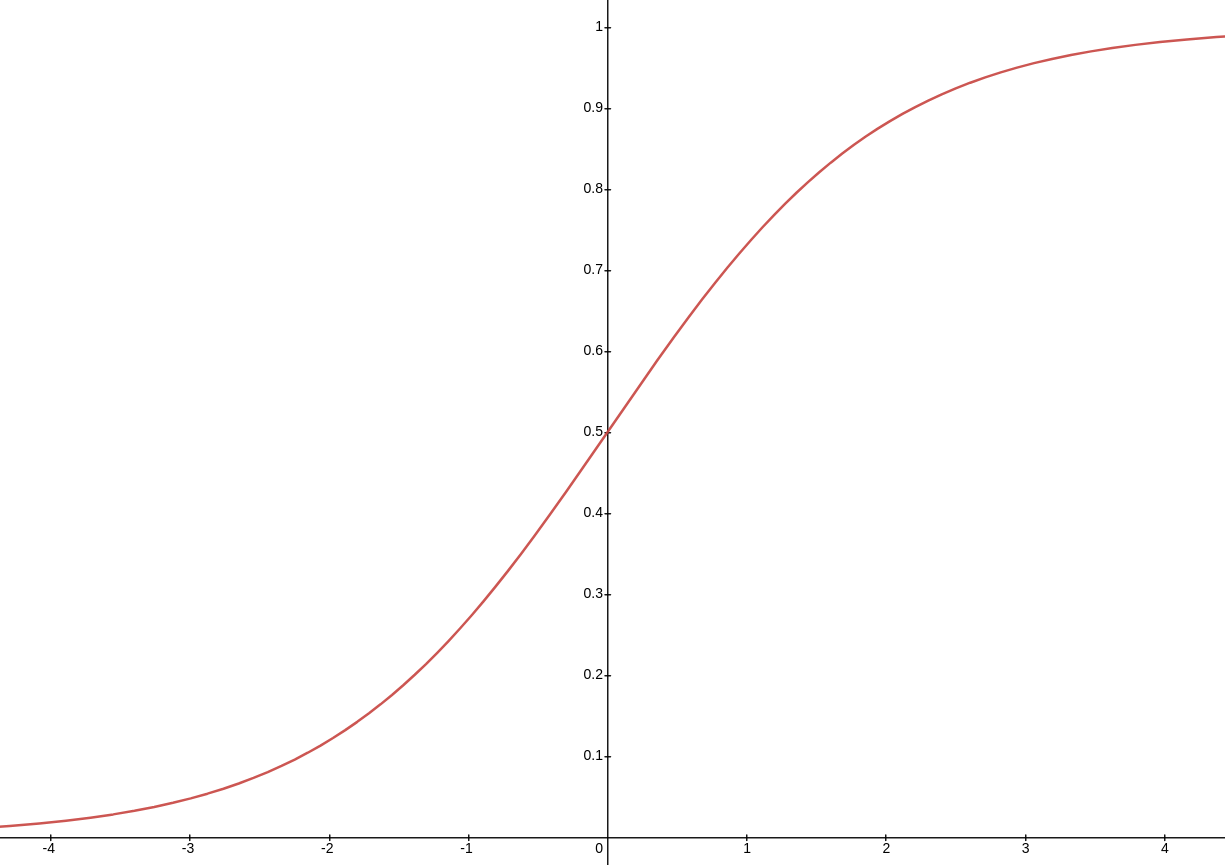
\includegraphics[width=0.5\textwidth]{sigmoid_small}
\caption[Simoid function]{
  \textbf{Sigmoid function.}
  The figures shows the plot of the logistic sigmoid function.
}
\label{fig:sigmoid}
\end{figure}

\begin{table}[h!] % positioning: here, enforced
\label{tab:example}
\center
\begin{tabular}{m{40mm}lllll}
  \toprule
  & bias & \# weights \\
  \midrule
  $Pol_1$ with bias & True & x \\
  $Pol_1$ without bias & False & x \\
  $Pol_2$ with bias & True & x \\
  $Pol_2$ without bias & False & x \\
  \bottomrule
  \end{tabular}
  \caption[Example]{%
    \textbf{Polynomial.}
    Description of structure of polynomial models.
  }
\end{table}


\section{Results}
\subsection{Experiment 1}


\subsubsection{Neural Network}

\subsubsection{Polynomial}

\section{Results}
